\chapter{Dettagli dei casi d'uso specifici}

\vspace{-1cm}

\section{Utente: Creazione di una nuova Issue}

\textit{\underline{Mockup}}

\begin{figure}[H]
  \centering
  \includegraphics[scale=0.2]{images/mockups/addIssue/progetto.pdf}
  \caption{UC02\_MC01}
\end{figure}

\begin{figure}[H]
  \centering
  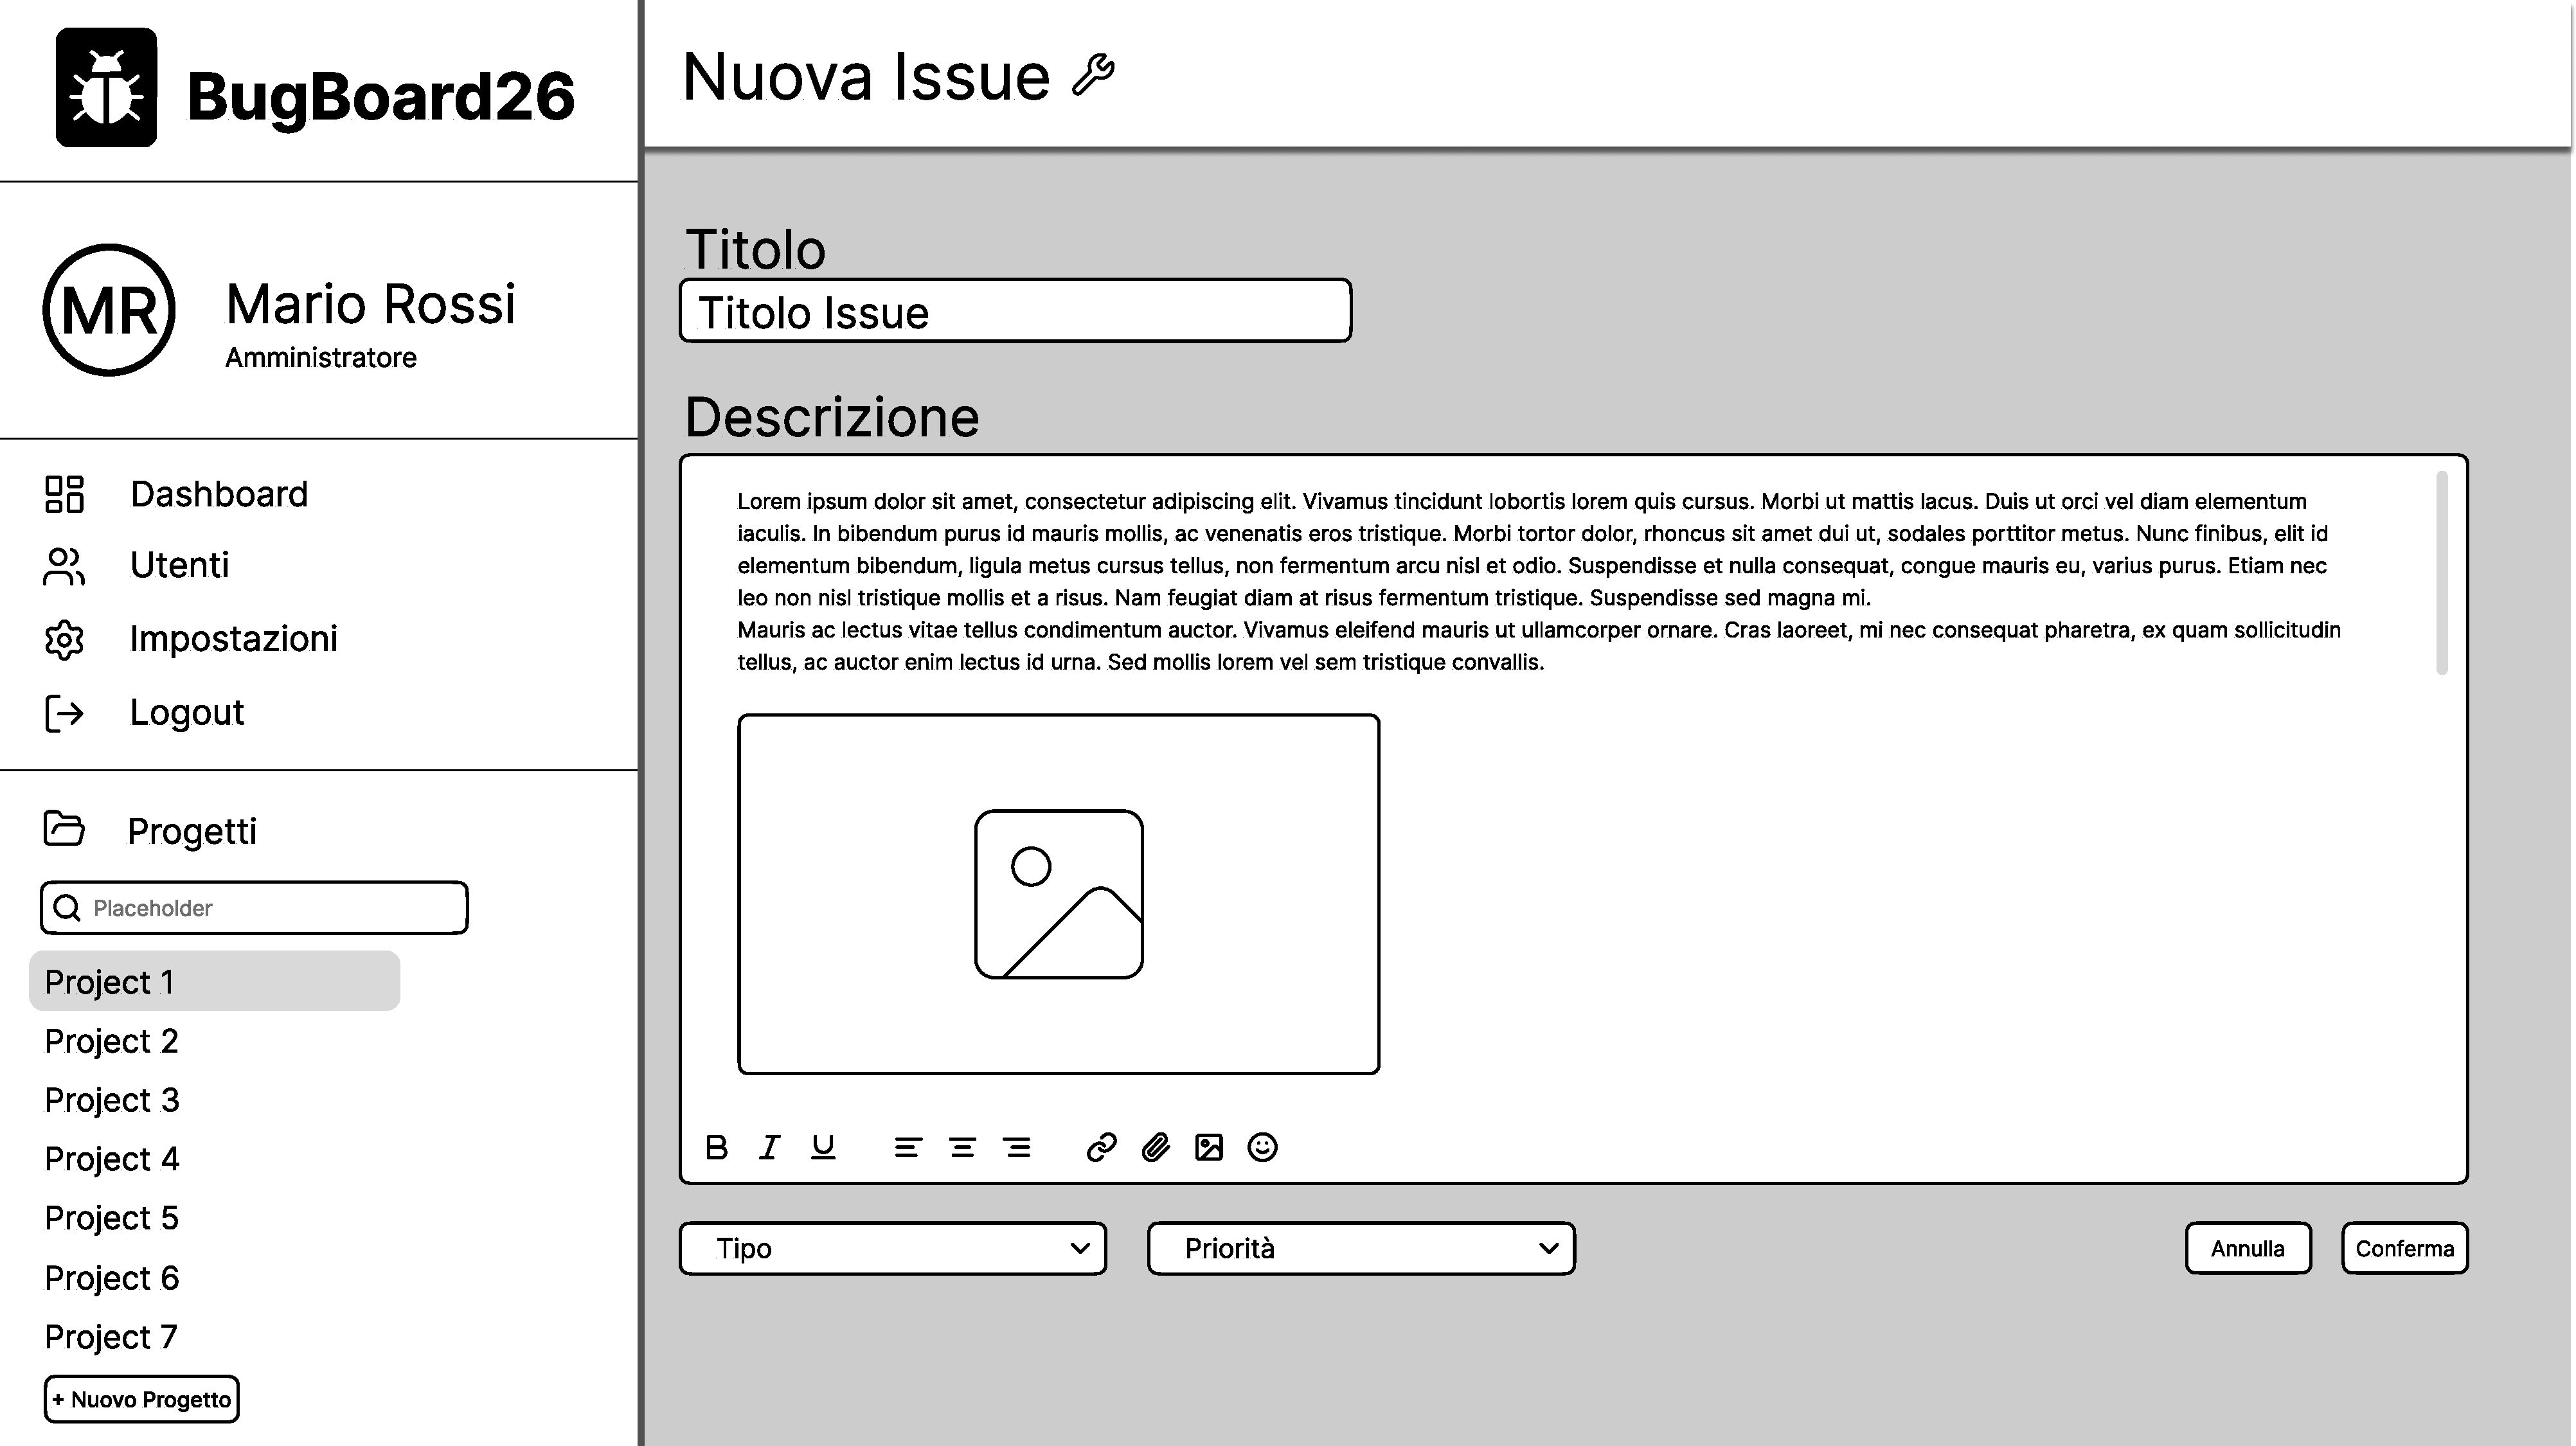
\includegraphics[scale=0.2]{images/mockups/addIssue/base.pdf}
  \caption{UC02\_MC02}
\end{figure}

\begin{figure}[H]
  \centering
  \includegraphics[scale=0.2]{images/mockups/addIssue/conferma.pdf}
  \caption{UC02\_MC03}
\end{figure}

\begin{figure}[H]
  \centering
  \includegraphics[scale=0.2]{images/mockups/addIssue/errore.pdf}
  \caption{UC02\_MC04}
\end{figure}

\newpage

\renewcommand{\arraystretch}{1.3}

\begin{longtable}{|>{\centering\arraybackslash\bfseries}p{3.5cm}|p{12cm}|}
  \hline
  \rowcolor{airforceblue!80!cyan}
  \textcolor{white}{\textbf{Use Case \#02}} & \textcolor{white}{\textbf{Crea Nuova Issue}} \\
  \hline
  \endfirsthead
  \endhead

  \rowcolor{beaublue!30}
  \textit{Scopo} & Un utente vuole creare una nuova Issue. \\ \hline
  Precondizioni & L'utente è autenticato nel sistema. \\ \hline
  \rowcolor{beaublue!30}
  \textit{Condizione finale di successo} & La nuova Issue è stata creata con successo nel sistema. \\ \hline
  Condizione finale di insuccesso & La creazione della nuova Issue non è riuscita a causa di un errore del sistema o di dati non validi forniti dall'utente. \\ \hline
  \rowcolor{beaublue!30}
  \textit{Attore Principale} & Utente generale \\ \hline
  Trigger & L'utente clicca sul bottone "Nuova Issue" in UC02\_MC01. \\ \hline

  \rowcolor{beaublue!30}
  \textit{Main Scenario} & \hspace{-0.37cm}
  \begin{minipage}{\linewidth}
    \renewcommand{\arraystretch}{1.1}
    \begin{tabular}{|c|p{5.2cm}|p{4.45cm}|}
      \hline
      \rowcolor{beaublue!30}
      \textbf{Step n.} & \textbf{Utente generale} & \textbf{Sistema} \\ \hline
      01 & L'utente clicca sul bottone "Nuova Issue" in UC02\_MC01 & \\ \hline
      \rowcolor{white}
      02 & & Il sistema mostra UC02\_MC02 \\ \hline
      \rowcolor{beaublue!30}
      03 & L'utente compila correttamente il form e clicca "Conferma" & \\ \hline
      \rowcolor{white}
      04 & & Mostra UC02\_MC03 \\ \hline
      \rowcolor{beaublue!30}
      05 & L'utente clicca sul bottone "Conferma" & \\ \hline
      \rowcolor{white}
      06 & & Mostra UC02\_MC01 e termina UC \\ \hline
    \end{tabular}
  \end{minipage} \\ \hline

  \textit{Extension \#01} & \hspace{-0.37cm}
  \begin{minipage}{\linewidth}
    \renewcommand{\arraystretch}{1.1}
    \begin{tabular}{|c|p{5.2cm}|p{4.45cm}|}
      \hline
      \rowcolor{beaublue!30}
      \textbf{Step n.} & \textbf{Utente generale} & \textbf{Sistema} \\ \hline
      3.01 & L'utente non compila titolo o descrizione e clicca "Conferma" & \\ \hline
      \rowcolor{white}
      4.01 & & Mostra UC02\_MC04 \\ \hline
      \rowcolor{beaublue!30}
      5.01 & L'utente clicca sul bottone "Conferma" & \\ \hline
      \rowcolor{white}
      6.01 & & Riparte dal punto 2 \\ \hline
    \end{tabular}
  \end{minipage} \\ \hline

  \rowcolor{beaublue!30}
  \textit{Extension \#02} & \hspace{-0.37cm}
  \begin{minipage}{\linewidth}
    \renewcommand{\arraystretch}{1.1}
    \begin{tabular}{|c|p{5.2cm}|p{4.45cm}|}
      \hline
      \rowcolor{beaublue!30}
      \textbf{Step n.} & \textbf{Utente generale} & \textbf{Sistema} \\ \hline
      3.02 & L'utente clicca sul bottone "Annulla" & \\ \hline
      \rowcolor{white}
      4.02 & & Mostra UC02\_MC01 e termina UC \\ \hline
    \end{tabular}
  \end{minipage} \\ \hline
\end{longtable}

\begin{longtable}{|>{\centering\arraybackslash\bfseries}p{3.5cm}|p{12cm}|}
  \hline
  \rowcolor{airforceblue!80!cyan}
  \textcolor{white}{\textbf{Codice}} & \textcolor{white}{\textbf{Requisito}} \\
  \hline
  \endfirsthead
  \endhead

  \rowcolor{beaublue!30}
  \textit{UR02\_01} & Il sistema deve permettere il caricamento di immagini o documenti pdf. Per un massimo di tre documenti, ciascuno con dimensione massima 5MB. \\ \hline
  \rowcolor{beaublue!30}
\end{longtable}

\newpage

\section{Amministratore: Aggiunta di un nuovo utente}

\begin{figure}[H]
  \centering
  \includegraphics[scale=0.2]{images/mockups/addUser/base.pdf}
  \caption{UC08\_MC01}
\end{figure}

\begin{figure}[H]
  \centering
  \includegraphics[scale=0.2]{images/mockups/addUser/form.pdf}
  \caption{UC08\_MC02}
\end{figure}

\begin{figure}[H]
  \centering
  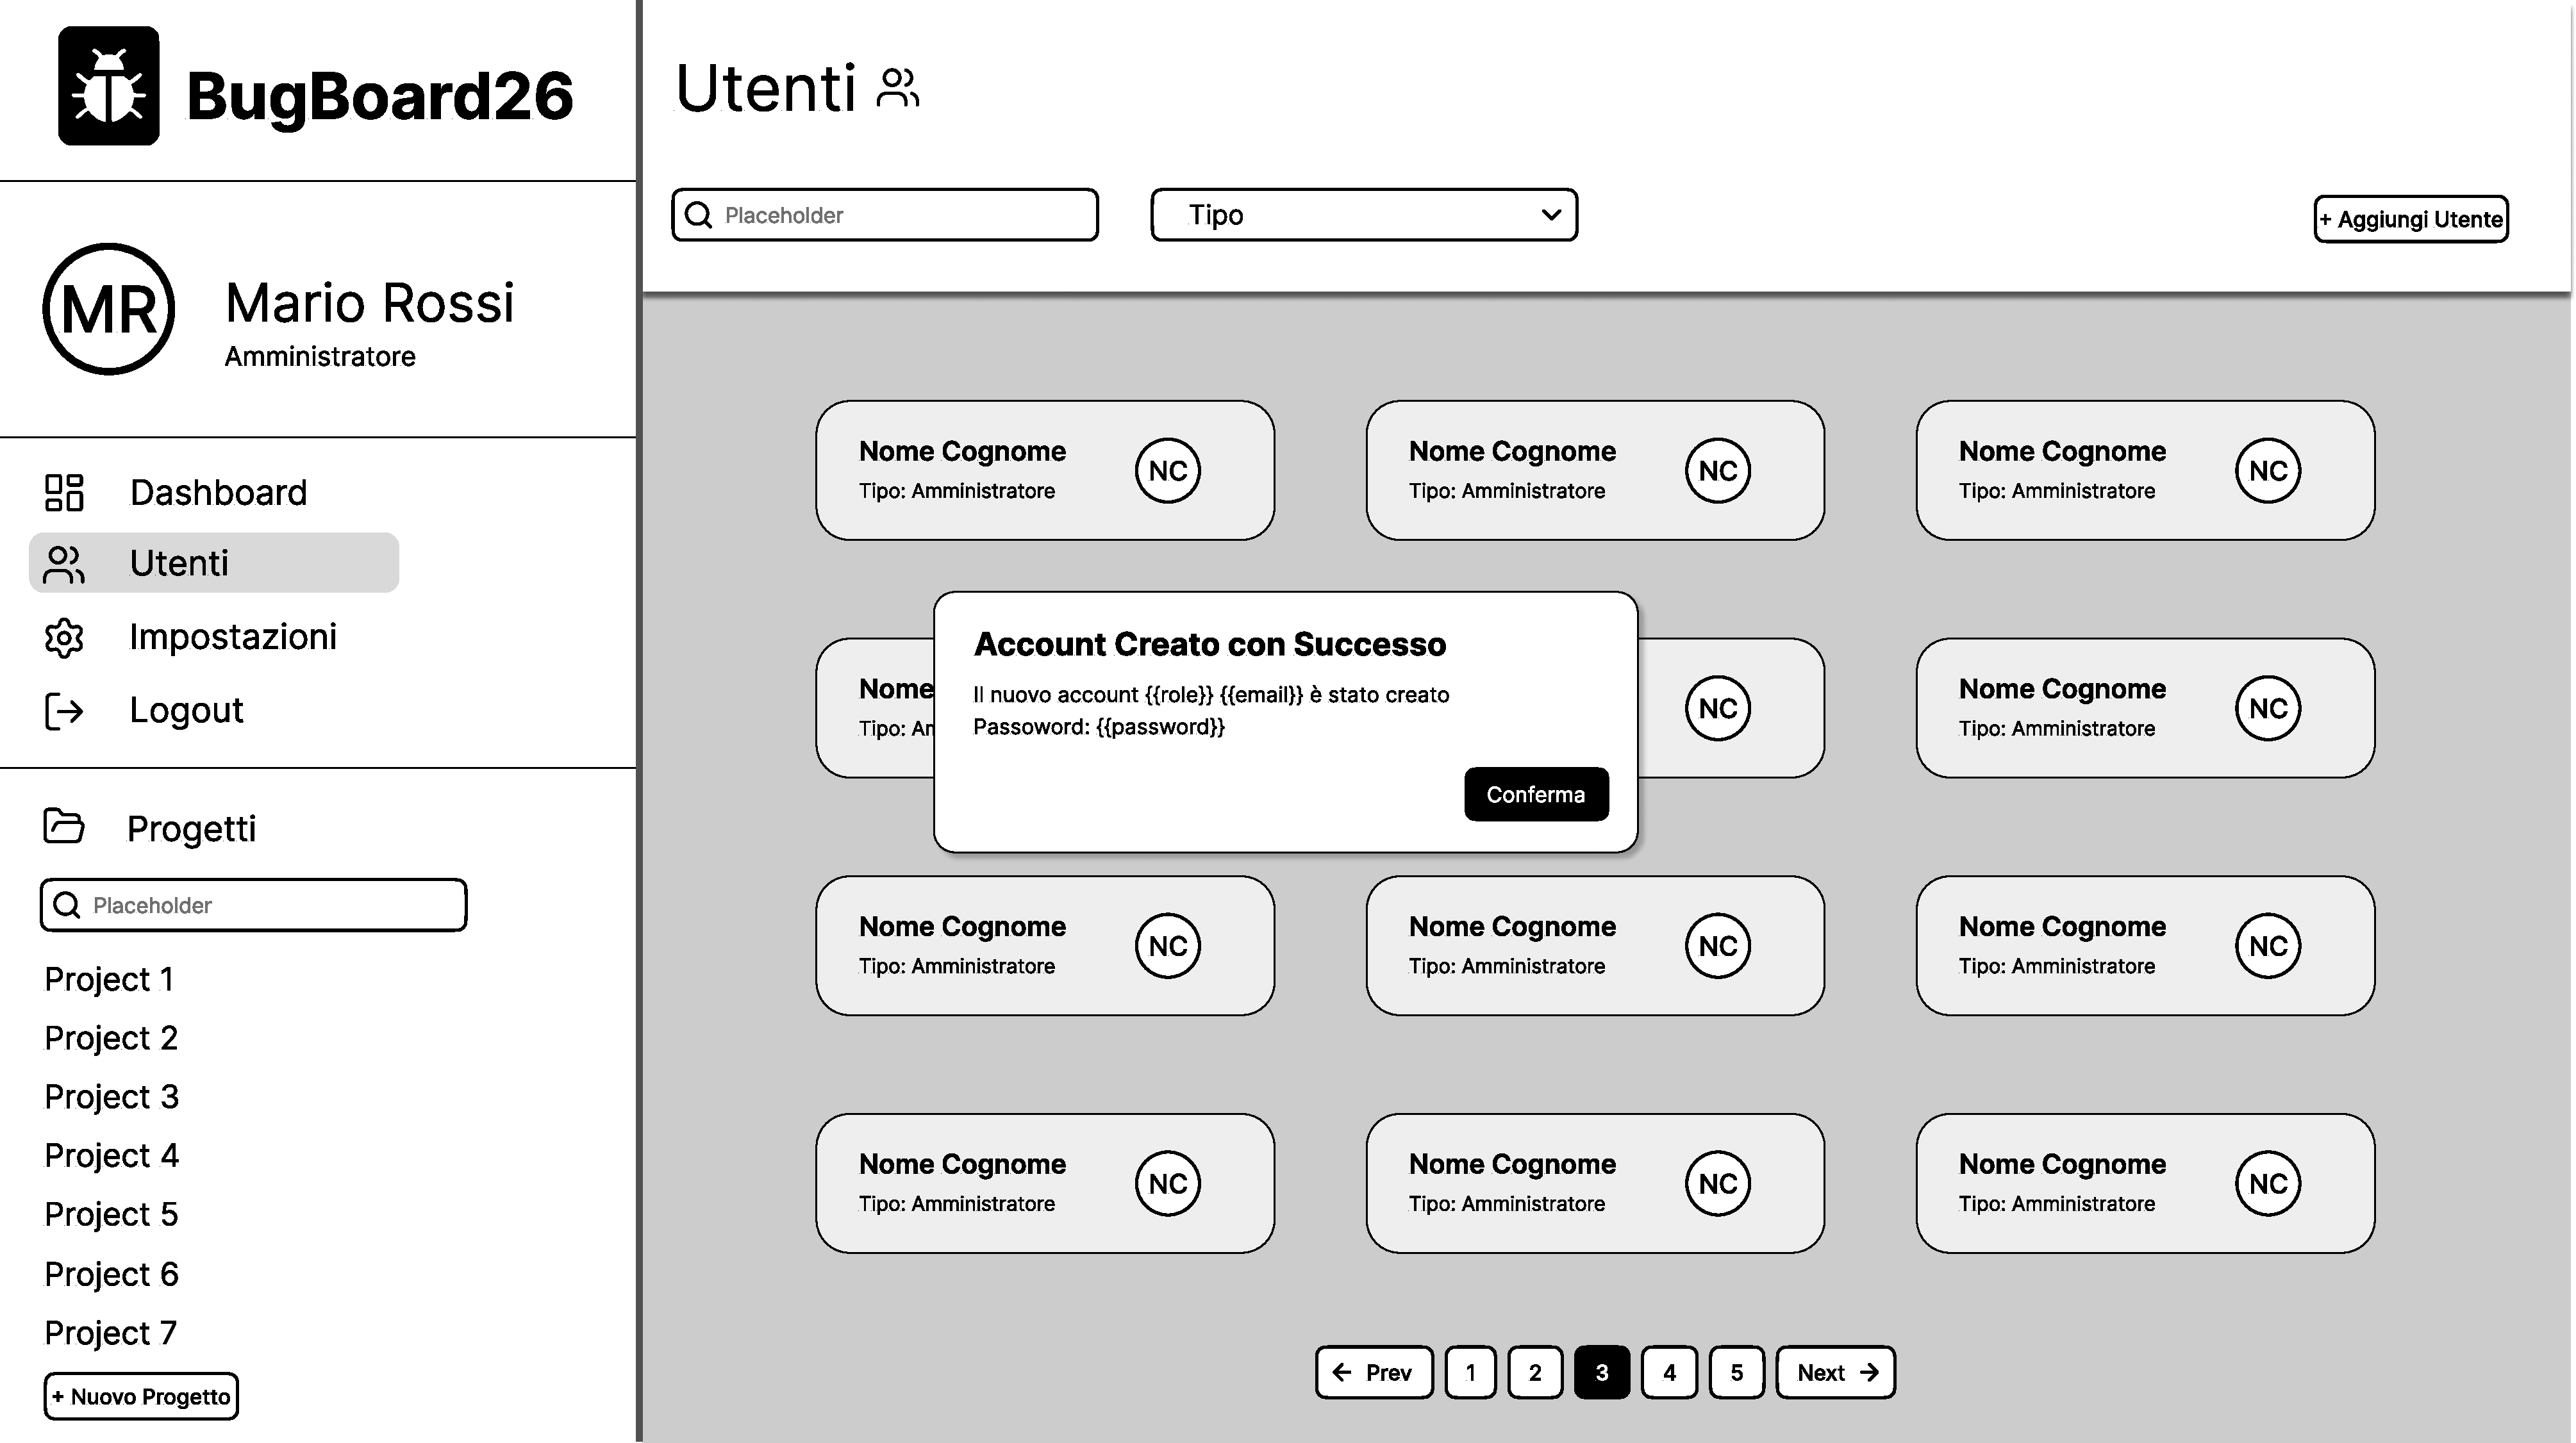
\includegraphics[scale=0.2]{images/mockups/addUser/success.pdf}
  \caption{UC08\_MC03}
\end{figure}

\begin{figure}[H]
  \centering
  \includegraphics[scale=0.2]{images/mockups/addUser/errore.pdf}
  \caption{UC08\_MC04}
\end{figure}

\newpage

\renewcommand{\arraystretch}{1.3}

\begin{longtable}{|>{\centering\arraybackslash\bfseries}p{3.5cm}|p{12cm}|}
  \hline
  \rowcolor{airforceblue!80!cyan}
  \textcolor{white}{\textbf{Use Case \#08}} & \textcolor{white}{\textbf{Aggiungi Nuovo Utente}} \\
  \hline
  \endfirsthead
  \endhead

  \rowcolor{beaublue!30}
  \textit{Scopo} & L'amministratore vuole aggiungere un nuovo utente. \\ \hline
  Precondizioni & L'amministratore è autenticato nel sistema. \\ \hline
  \rowcolor{beaublue!30}
  \textit{Condizione finale di successo} & Il nuovo utente è stato aggiunto con successo nel sistema. \\ \hline
  Condizione finale di insuccesso & L'aggiunta del nuovo utente non è riuscita a causa di un errore del sistema o di dati non validi forniti dall'amministratore. \\ \hline
  \rowcolor{beaublue!30}
  \textit{Attore Principale} & Amministratore. \\ \hline
  Trigger & L'amministratore clicca sul bottone "Nuovo Utente" in UC08\_MC01. \\ \hline

  \rowcolor{beaublue!30}
  \textit{Main Scenario} & \hspace{-0.37cm}
  \begin{minipage}{\linewidth}
    \renewcommand{\arraystretch}{1.1}
    \begin{tabular}{|c|p{5.2cm}|p{4.45cm}|}
      \hline
      \rowcolor{beaublue!30}
      \textbf{Step n.} & \textbf{Amministratore} & \textbf{Sistema} \\ \hline
      01 & L'amministratore clicca sul bottone "Aggiungi Utente" in UC08\_MC01 & \\ \hline
      \rowcolor{white}
      02 & & Il sistema mostra UC08\_MC02 \\ \hline
      \rowcolor{beaublue!30}
      03 & L'amministratore inserisce nome, cognome, ruolo, email e clicca "Conferma" & \\ \hline
      \rowcolor{white}
      04 & & Mostra UC08\_MC03 \\ \hline
      \rowcolor{beaublue!30}
      05 & L'amministratore clicca sul bottone "Continua" & \\ \hline
      \rowcolor{white}
      06 & & Mostra UC08\_MC01 e termina UC \\ \hline
    \end{tabular}
  \end{minipage} \\ \hline

  \textit{Extension \#01} & \hspace{-0.37cm}
  \begin{minipage}{\linewidth}
    \renewcommand{\arraystretch}{1.1}
    \begin{tabular}{|c|p{5.2cm}|p{4.45cm}|}
      \hline
      \rowcolor{beaublue!30}
      \textbf{Step n.} & \textbf{Amministratore} & \textbf{Sistema} \\ \hline
      3.01 & L'amministratore clicca sul bottone "Annulla" & \\ \hline
      \rowcolor{white}
      4.01 & & Mostra UC08\_MC01 e termina UC \\ \hline
    \end{tabular}
  \end{minipage} \\ \hline

  \rowcolor{beaublue!30}
  \textit{Extension \#02} & \hspace{-0.37cm}
  \begin{minipage}{\linewidth}
    \renewcommand{\arraystretch}{1.1}
    \begin{tabular}{|c|p{5.2cm}|p{4.45cm}|}
      \hline
      \rowcolor{beaublue!30}
      \textbf{Step n.} & \textbf{Amministratore} & \textbf{Sistema} \\ \hline
      3.02 & L'amministratore compila il form con un'email già esistente e clicca "Conferma" & \\ \hline
      \rowcolor{white}
      4.02 & & Mostra UC08\_MC04 \\ \hline
      \rowcolor{beaublue!30}
      5.02 & L'amministratore clicca sul bottone "Conferma" & \\ \hline
      \rowcolor{white}
      6.02 & & Riparte dal punto 2  \\
    \end{tabular}
  \end{minipage} \\ \hline
\end{longtable}

\begin{longtable}{|>{\centering\arraybackslash\bfseries}p{3.5cm}|p{12cm}|}
  \hline
  \rowcolor{airforceblue!80!cyan}
  \textcolor{white}{\textbf{Codice}} & \textcolor{white}{\textbf{Requisito}} \\
  \hline
  \endfirsthead
  \endhead

  \rowcolor{beaublue!30}
  \textit{UR08\_01} & Il sistema deve essere in grado di controllare la formattazione dell'email \\ \hline
  \rowcolor{beaublue!30}
\end{longtable}

\newpage

\section{Utente: Aggiunta di un commento a una Issue esistente}

\begin{figure}[H]
  \centering
  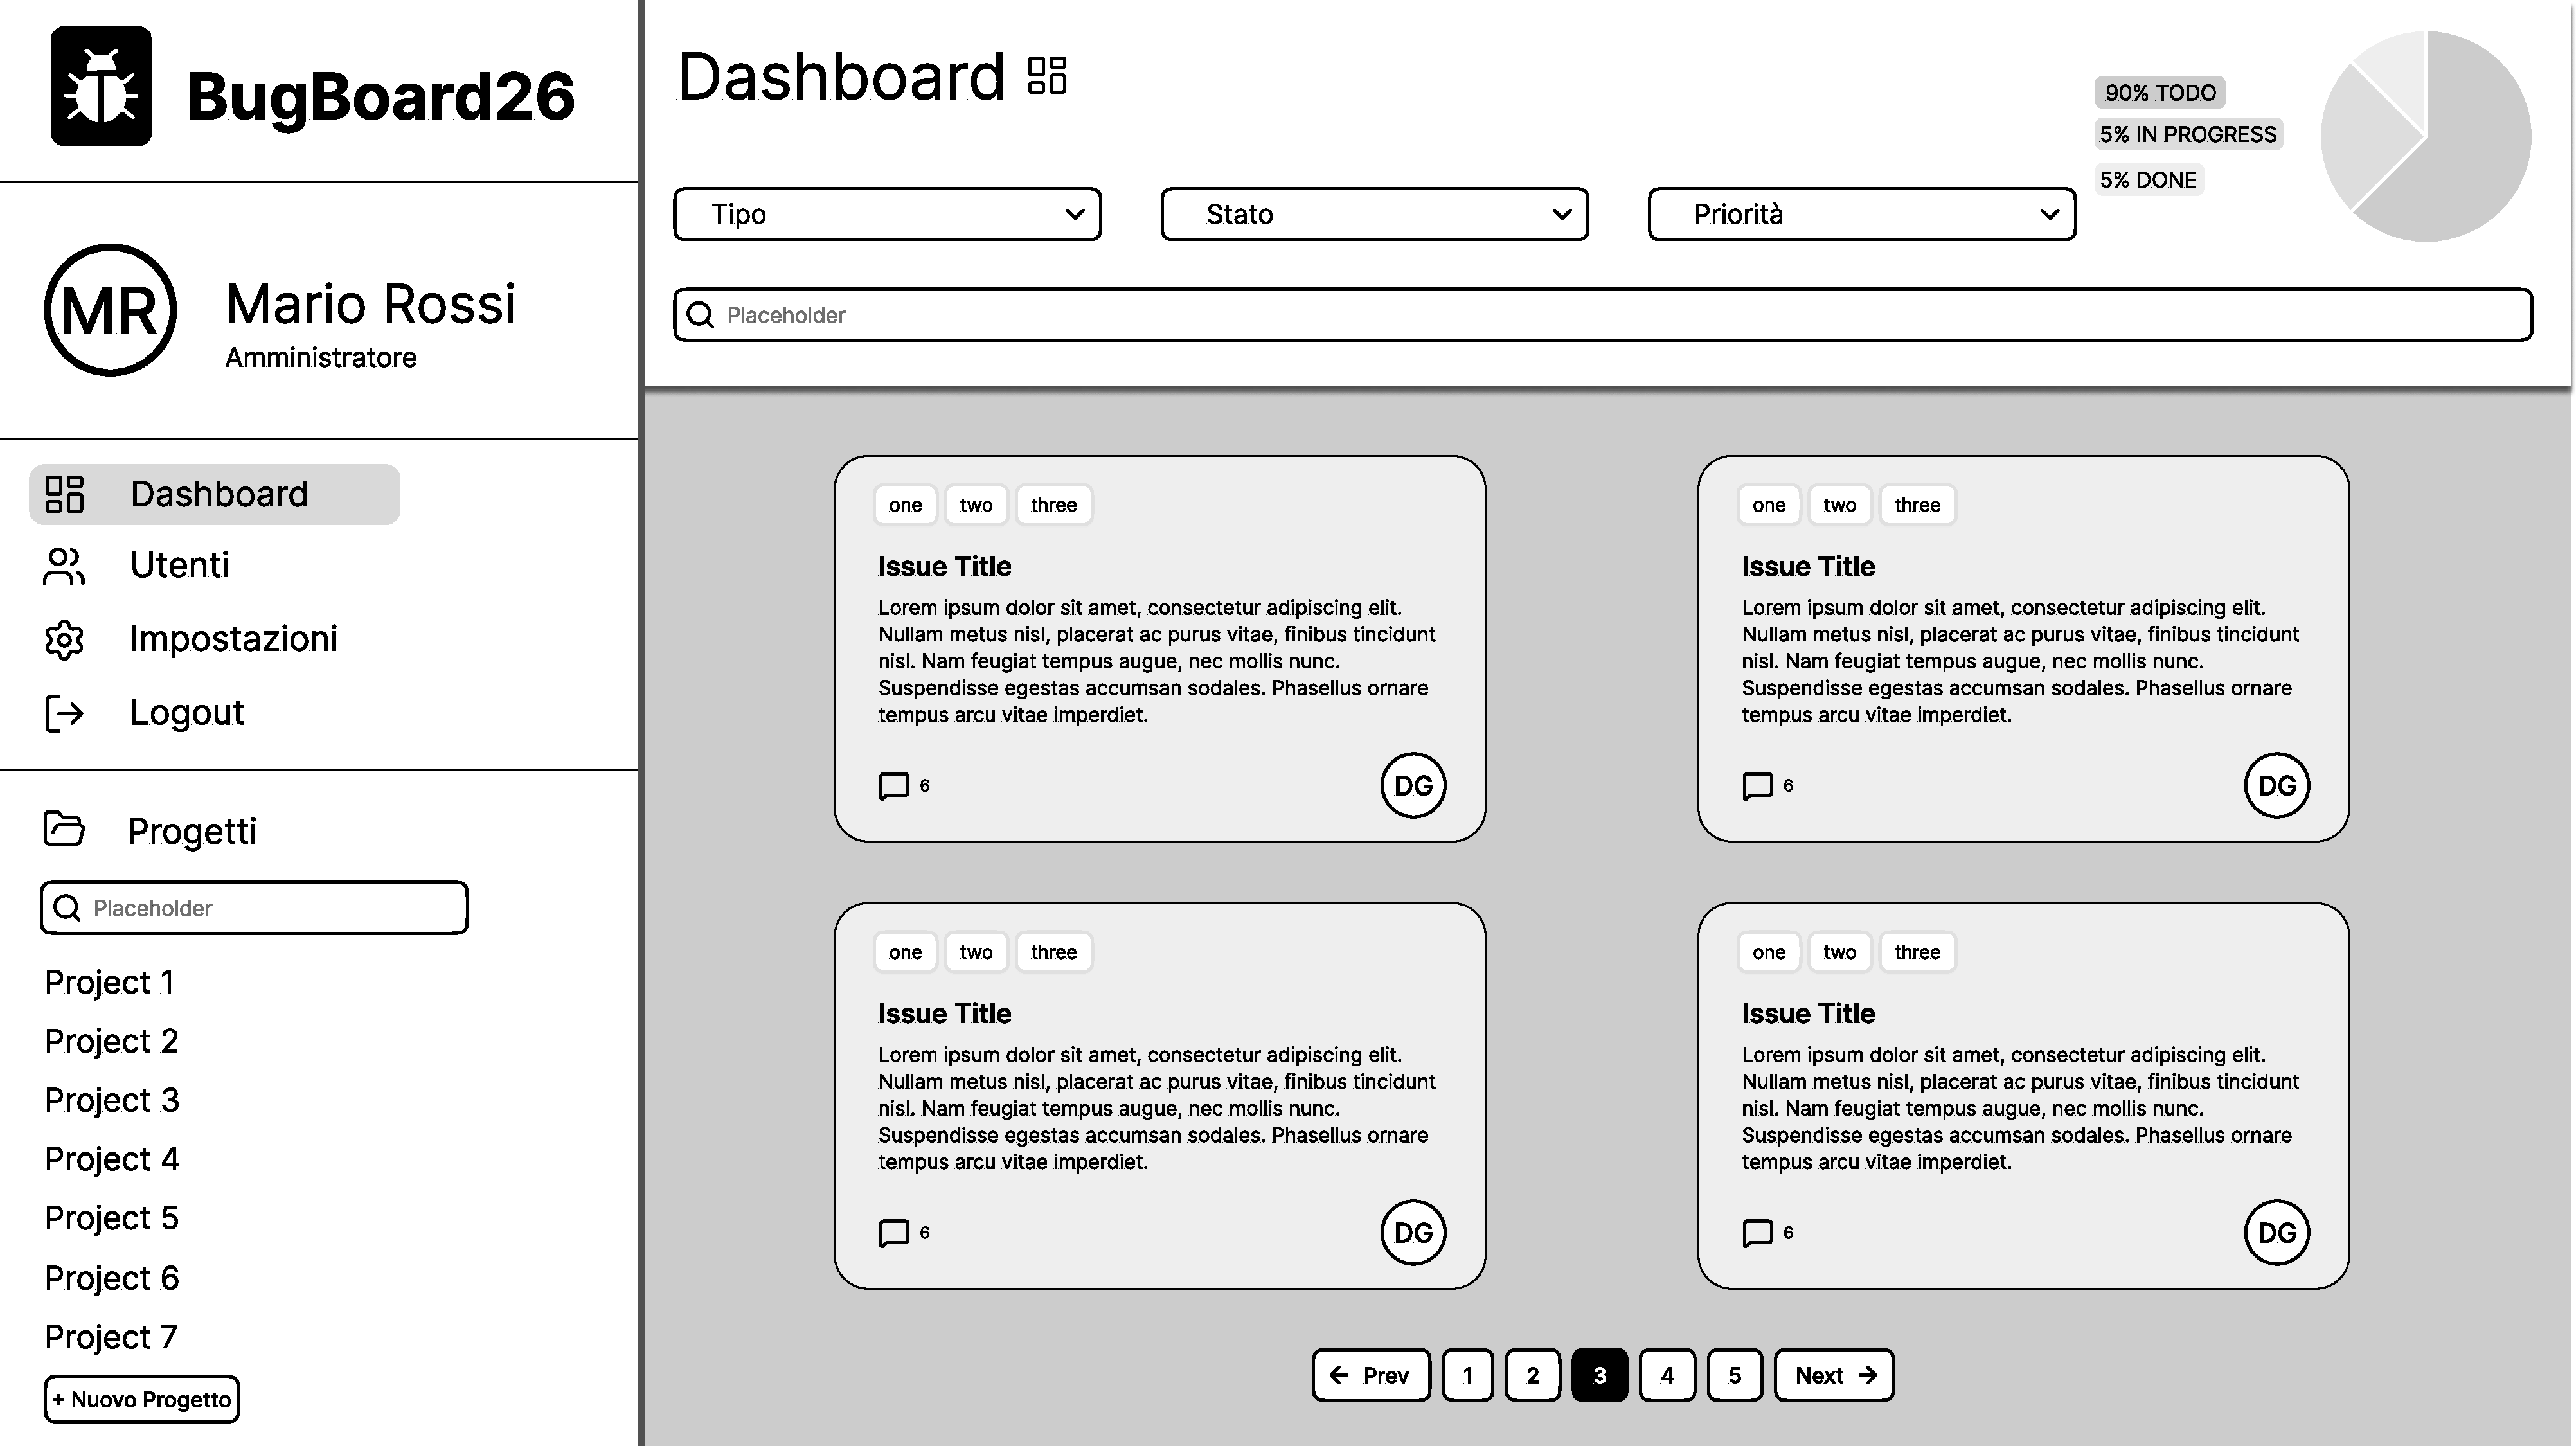
\includegraphics[scale=0.2]{images/mockups/addComment/dashboard.pdf}
  \caption{UC05\_MC01}
\end{figure}

\begin{figure}[H]
  \centering
  \includegraphics[scale=0.2]{images/mockups/addComment/progetto.pdf}
  \caption{UC05\_MC02}
\end{figure}

\begin{figure}[H]
  \centering
  \includegraphics[scale=0.2]{images/mockups/addComment/base.pdf}
  \caption{UC05\_MC03}
\end{figure}

\newpage

\renewcommand{\arraystretch}{1.3}

\begin{longtable}{|>{\centering\arraybackslash\bfseries}p{3.5cm}|p{12cm}|}
  \hline
  \rowcolor{airforceblue!80!cyan}
  \textcolor{white}{\textbf{Use Case \#05}} & \textcolor{white}{\textbf{Aggiungi Commento a Issue}} \\
  \hline
  \endfirsthead
  \endhead

  \rowcolor{beaublue!30}
  \textit{Scopo} & L'utente vuole aggiungere un commento a una issue esistente. \\ \hline
  Precondizioni & L'utente è autenticato nel sistema. \\ \hline
  \rowcolor{beaublue!30}
  \textit{Condizione finale di successo} & Il commento è stato aggiunto con successo alla issue. \\ \hline
  Condizione finale di insuccesso & L'aggiunta del commento non è riuscita a causa di un errore del sistema o di dati non validi forniti dall'utente. \\ \hline
  \rowcolor{beaublue!30}
  \textit{Attore Principale} & Utente. \\ \hline
  Trigger & L'utente si trova in UC05\_MC01 oppure in UC05\_MC02 e visualizza un'issue. \\ \hline

  \rowcolor{beaublue!30}
  \textit{Main Scenario} & \hspace{-0.37cm}
  \begin{minipage}{\linewidth}
    \renewcommand{\arraystretch}{1.1}
    \begin{tabular}{|c|p{5.2cm}|p{4.45cm}|}
      \hline
      \rowcolor{beaublue!30}
      \textbf{Step n.} & \textbf{Utente} & \textbf{Sistema} \\ \hline
      01 & L'utente clicca su una issue per visualizzarla in UC05\_MC01 o UC05\_MC02 & \\ \hline
      \rowcolor{white}
      02 & & Il sistema mostra UC05\_MC03 \\ \hline
      \rowcolor{beaublue!30}
      03 & L'utente compila la textbox dedicata e clicca "Commenta" & \\ \hline
      \rowcolor{white}
      04 & & Mostra il commento in UC05\_MC03 e termina UC \\ \hline
    \end{tabular}
  \end{minipage} \\ \hline
\end{longtable}

\begin{longtable}{|>{\centering\arraybackslash\bfseries}p{3.5cm}|p{12cm}|}
  \hline
  \rowcolor{airforceblue!80!cyan}
  \textcolor{white}{\textbf{Codice}} & \textcolor{white}{\textbf{Requisito}} \\
  \hline
  \endfirsthead
  \endhead

  \rowcolor{beaublue!30}
  \textit{UR05\_01} & Il sistema deve permettere il caricamento di immagini o documenti pdf. Per un massimo di tre documenti, ciascuno con dimensione massima 5MB. \\ \hline
  \rowcolor{beaublue!30}
\end{longtable}